
\chapter{Interacciones y movimiento}

 
\section{Diagramas mostrando cambios de velocidad}

Está parte de la notas está basada en el libro Matter \& Interactions \cite{MI}

En diagrámas físicaos la velocidad de un objeto es representada por un
vector: una línea con una flecha. La cola de la flecha se coloca donde
el objeto está localizado, y la punta de la flecha en la dirección del
movimiento del objeto. La longitud de la flecha es proporcional a la
velocidad del objeto. De este modo la velocidad se describe como un
vector. A la magnitud de la velocidad se le llama rapidez.

\subsection{Movimiento uniforme}
Suponga que observa una roca moviéndose en el espacio exterior
bastante alejada de cualquier objeto. No sabemos que la hizo mover la
primera vez; presumiblemente hace mucho tiempo una interacción de dio
alguna velocidad y esta ha estado moviéndose desde entonces en el
espacio vacio.

Es un hecho observacional que tal objeto aislado se mueve con una
rapidez constante (que no cambia), en una línea recta. Su velocidad no
cambia (ni su dirección ni su rapidez
\begin{figure}
  \centering
  \includegraphics[scale=0.3]{uniform}
  \caption{Movimiento uniforme: sin cambio en la rapidez o la dirección.}
  \label{fig:uniform}
\end{figure}
cambia). A tal movimiento con
velocidad constante le llamaremos movimiento uniforme y es ilustrado
en la figura~\ref{fig:uniform}

Ver presentación sobre Interacciones y movimiento donde se establece la Primera Ley de Newton en la página del curso.

\section{Velocidad}

\subsection{Rapidez promedio}
La rapidez es un número y por consiguiente es una cantidad escalar:

\begin{align}
  \label{eq:27}
\bar{v}=\frac{d}{t}
\end{align}
donde $\bar{v}$ es la \emph{rapidez promedio}, $d$ es la distancia
recorrida durante un tiempo $t$. En SI (Système Internationale) de
unidades, la rapidez promedio se mide en metros por segundo, y se
abrevia con $m/s$.

De \eqref{eq:27}
\begin{align}
  \label{eq:26}
  d=&\bar{v} t\nonumber\\
  t=&\frac{d}{\bar{v}}
\end{align}

Es importante notar que las ecuaciones \eqref{eq:26} son dimensionalmente correctas, por ejemplo
\begin{align}
  [d]=&  \left[\bar{v}   \right] [t]\nonumber\\
  L=&\frac{L}{T}\times T\nonumber\\
  L=&L
\end{align}

\subsection{Rapidez instantanea comparada a rapidez promedio}

Si un carro se mueve a $70\ \text{Km/h}$ (Kolometros por hora) durante la primera hora y a $30\ \text{Km/h}$
durante la segunda hora, este recorre en total 100~Km en 2 horas, con una velocidad promedio
\begin{align}
  \bar{v}=\frac{100\ \text{Km}}{2\ \text{h}}=50\ \text{Km/h}\,.
\end{align}
Note que durante el intervalo de dos horas el carro nunca fue viajando realmente a su velocidad promedio de 50~Km/h.

El movimiento es ilustrado en un gráfico de distancia contra tiempo en la figura~\ref{fig:vinstaprom3} (detalles en la presentación \href{http://goo.gl/3eqUa}{aquí})

\begin{frame}[plain]
\begin{figure}
  \centering
  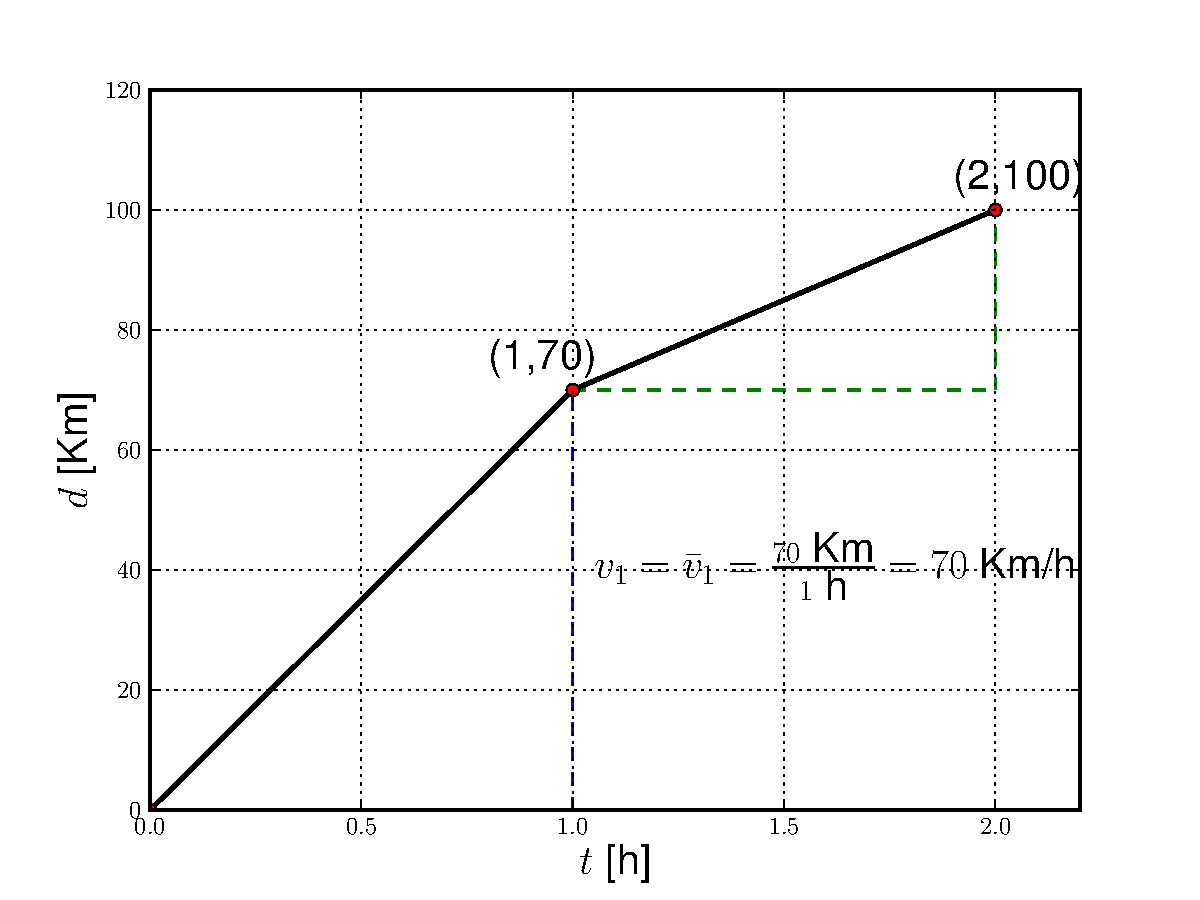
\includegraphics[scale=0.6]{vinstaprom3}
  \caption{Grafico de distancia versus tiempo}
  \label{fig:vinstaprom3}
\end{figure}
\end{frame}


La rapidez instantánea es la rapidez del carro en un instante particular. Para encontrarla debemos observar una distancia corta que el carro se mueva en un intervalo de tiempo muy corto, digamos que una centesima de segundo. Si durante algún momento de la segunda hora el carro se mueve 0.0833 metros en 0.01 segundos, su rapidez instantanea es:
\begin{align}
  v=0.0833/0.01=8.33 m/s\,,
\end{align}
que en Km/h corresponde a
\begin{align}
  v=8.33\ \frac{\cancel{\text{m}}}{\cancel{\text{s}}}\frac{3600\ \cancel{\text{s}}}{1h}\frac{1\ \text{Km}}{1000\ \cancel{\text{m}}}=30\ \frac{\text{Km}}{\text{h}}\,.
\end{align}



\section{Movimiento en varias dimensiones}

\subsection{Vector de Posici\'on}
Nuestra segunda aplicaci\'on de vectores ser\'a la descripci\'on  de la posici\'on y movimiento de un punto en el espacio en tres dimensiones. 

La posici\'on de un punto en el espacio: $(x_1,y_1,z_1)$ no representa un vector. Sin embargo, si movemos el punto a alguna nueva posici\'on, $(x_2,y_2,z_2)$, entonces el desplazamiento define un vector 
\begin{align}
  \Delta \mathbf{r}=\mathbf{r}_2-\mathbf{r}_1
\end{align}
$\Delta r$ significa ``cambio de $\mathbf{r}$'' o $\mathbf{r}_2-\mathbf{r}_1$ (desplazamiento)

$\Delta t$ significa ``cambio de $t$'' or $t_2-t_1$ (intervalo de tiempo)

El símbolo $\Delta$ (delta) siempre significa ``final menos inicial''

\begin{align}
  \Delta\mathbf{r}=(x_2-x_1,y_2-y_1,z_2-z_1)\,.
\end{align}
$\Delta\mathbf{r}$ es un vector verdadero, aunque los valores de la coordenadas inicial y final dependen del sistema de coordenadas, $\Delta\mathbf{r}$ no depende del sistema de coordenadas. 

$\Delta\mathbf{r}$ tiene las dimensiones f\'\i sicas de longitud. 

%hablar de un ejemplo concreto como el de la abeja de MI Fig. 1.31

El vector de desplazamiento apunta desde la posición inicial hacia la posición final (final menos incial).

%calcular el desplazamiento númerico de la abeja

Aunque los vectores definen desplazamientos en lugar de posiciones, es posible describir la posici\'on de un punto con respecto al origen de un sistema de coordenadas dado por un vector especial, conocido como el \emph{vector de posici\'on}, que se extiende desde el origen hasta el punto de inter\'es. Usaremos el s\'\i mbolo $\mathbf{r}$ para denotar el vector de posici\'on. La posici\'on de un punto arbitrario $P$ se escribe como
\begin{align}
  \mathbf{r}=(x,y,z)=x\hat{\mathbf{i}}+
  y\hat{\mathbf{j}}+z\hat{\mathbf{k}}\,.
\end{align}

A diferencia de los vectores ordinarios, $\mathbf{r}$ depende del sistema de coordenadas. Si $\mathbf{R}$ es el vector desde el origen de un sistema de coordenadas no primado al origen de un sistema de coordenadas primado, tenemos
\begin{inprogress}
  Escribir los detalles...
\end{inprogress}
\begin{align}
  \mathbf{r}'=\mathbf{r}-\mathbf{R}\,.
\end{align}
Un verdadero  vector es independiente del sistema de coordenadas. Como se muestra en la figura~\ref{fig:vpos},
\begin{align}
  \Delta\mathbf{r}=&\mathbf{r}_2-\mathbf{r}_1\nonumber\\
  =&\mathbf{\mathbf{r}_2'+\mathbf{R}}
-\mathbf{\mathbf{r}_1'+\mathbf{R}}\nonumber\\
=&\mathbf{r}_2'-\mathbf{r}'_1\,.
\end{align}
\begin{frame}[plain]
  \begin{figure}
  \centering
  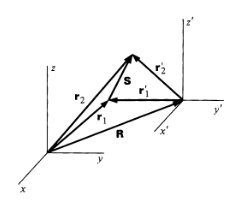
\includegraphics[scale=0.85]{vpos}
  \caption{Vector de desplazamiento. (Sec 1.6 \cite{Kleppner})}
  \label{fig:vpos}
\end{figure}
\end{frame}

\subsection{Determinando la velocidad promedio desde un cambio en la posición}
La posici\'on instant\'anea de una part\'\i cula a un tiempo $t_i$ es
\begin{align}
  \mathbf{r}(t_1)=(x(t_1),y(t_1),z(t_1))\qquad \text{\'o}\qquad
  \mathbf{r}_1=(x_1,y_1,z_1)\,,
\end{align}
donde $x_1$ es el valor de $x$ en $t=t_1$, y as\'\i{} sucesivamente. Al tiempo $t_2$ la posici\'on es
\begin{align}
  \mathbf{r}_2=(x_2,y_2,z_2)\,.
\end{align}
El desplazamiento de la part\'\i cula entre los tiempos $t_1$ y $t_2$ es
\begin{align}
  \mathbf{r}_2-\mathbf{r}_1=(x_2-x_1,y_2-y_1,z_2-z_1)\,.
\end{align}



\begin{inprogress}
Pasar las notas del cuaderno de MI aquí.

Escribir los detalles %t_1=t Delta t=t_2-t-> t_2=t+Delta t
\end{inprogress}
El desplazamiento de una part\'\i cula entre los tiempos $t$ y un tiempo posterior $t+\Delta t$ es
\begin{align}
  \Delta\mathbf{r}=\mathbf{r}(t+\Delta t)-\mathbf{r}(t)\,.
\end{align}


\begin{inprogress}
  Fig pag 15 of Kleppner.
\end{inprogress}

\begin{itemize}
\item[Ejemplo]: En dos dimensiones, esta ecuaci\'on es equivalente a
  \begin{align}
    \Delta x=&x(t+\Delta t)-x(t)\nonumber\\
    \Delta y=&y(t+\Delta t)-y(t)\,.
  \end{align}
  como se muestra en la figura~\cite{fig:deltar}
  \begin{figure}
    \centering
    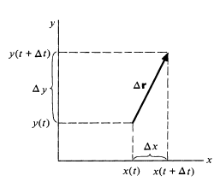
\includegraphics[scale=0.55]{deltar}
    \caption{Desplazamieto entre $t_1$ y $t_2$ (Sec 1.6~\cite{Kleppner})}
    \label{fig:deltar}
  \end{figure}

\end{itemize}

\subsection{Velocidad instantánea}

La curva en la figura \ref{fig:flyingball1a}. Los punto de color rojo marcan la posición de la bola a intervalos de tiempo de un segundo. Mientras que la bola está en el aire, su velocidad está constantemente cambiando, debido a las interacciones con la tierra (gravedad) y con el aire (resistencia del aire). 
\begin{figure}
  \centering
  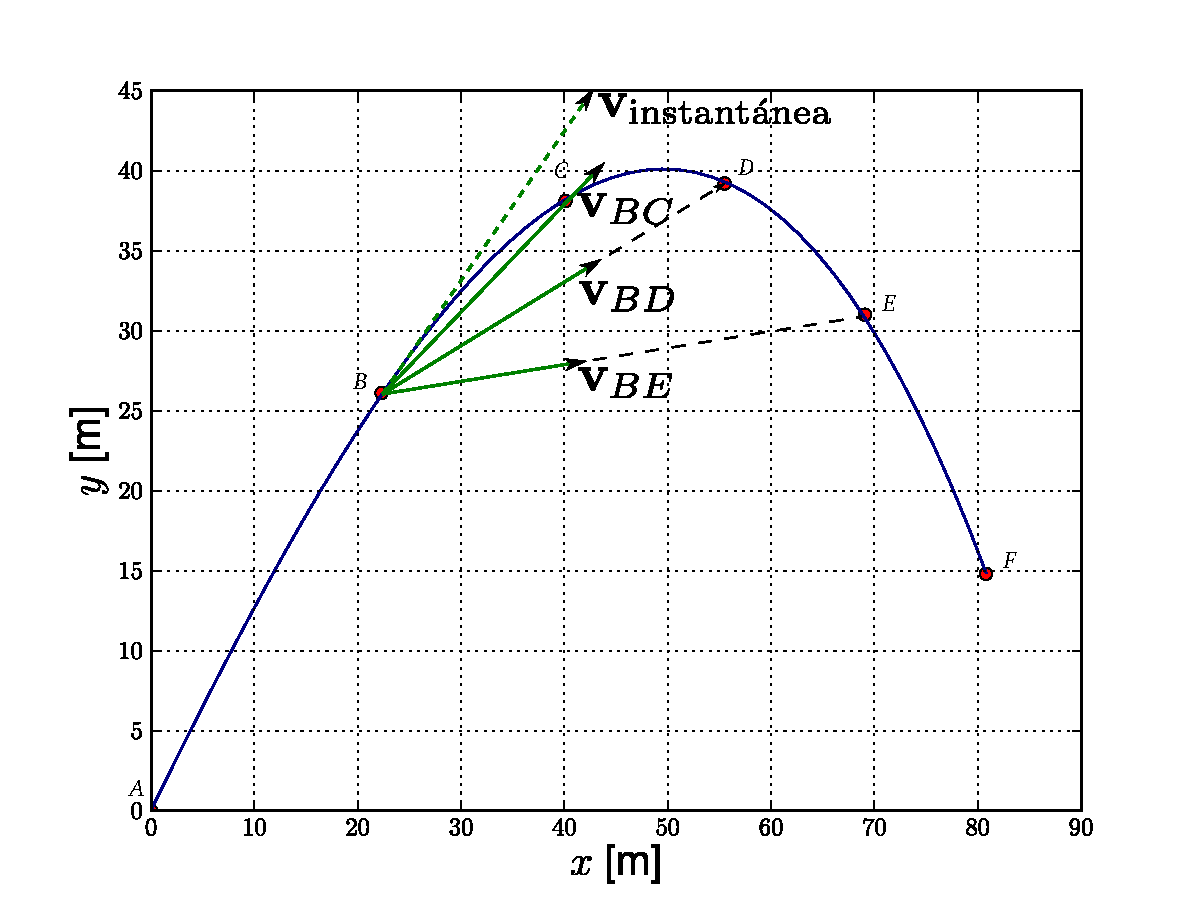
\includegraphics[scale=0.6]{flyingball1a}
  \caption{Moviemto de una bola}
  \label{fig:flyingball1a}
\end{figure}

Suponga que hacemos la pregunta: ¿cual es el valor de la velocidad en el instante preciso que alcanza el punto $B$?. Está cantidad debería llamarse la velocidad instantánea. Podemos aproximar la velocidad instantánea de la bola, encontrando su velocidad promedio sobre un intervalo de tiempo más grande. 

La Tabla

\begin{table}
  \centering
  \begin{tabular}{|l|l|l|}
    loc. & $t\ (\text{s})$ & Posición (m)\\
    $A$ & $0.0$ &$0,0,0$ \\
    $B$ & $1.0$ &$(22.3,26,1,0)$ \\
    $C$ & $2.0$ &$(40.1,38.1,0)$ \\
    $D$ & $3.0$ &$(55.5,39.2,0)$ \\
    $E$ & $4.0$ &$(69.1,31.0,0)$ \\
    $F$ & $5.0$ &$(80.8,14.8,0)$ \\
  \end{tabular}
  \caption{Tabla mostranto el tiempo transcurriod y la posición de la bola en cada posición de la figura \ref{fig:flyingball1a}}
  \label{tab:flyingball1a}
\end{table}

\begin{align}
  \mathbf{v}_{EB}=&\frac{\Delta \mathbf{r}_{EB}}{\Delta t}
=\frac{\mathbf{\mathbf{r}_E-\mathbf{r}_B}}{t_E-t_B}=
\frac{[(69.1,31.0,0)-(22.3,26,1,0)]\ \text{m}}{(4.0-1.0)\ \text{s}}\nonumber\\
=&(15.6,1.6,0)\ \frac{\text{m}}{\text{s}}\nonumber\\
  \mathbf{v}_{DB}=&\frac{\Delta \mathbf{r}_{DB}}{\Delta t}
=\frac{\mathbf{\mathbf{r}_D-\mathbf{r}_B}}{t_D-t_B}=
\frac{[(55.5,39.2,0)-(22.3,26,1,0)]\ \text{m}}{(3.0-1.0)\ \text{s}}\nonumber\\
=&(16.6,6.55,0)\ \frac{\text{m}}{\text{s}}\nonumber\\
  \mathbf{v}_{CB}=&\frac{\Delta \mathbf{r}_{CB}}{\Delta t}
=\frac{\mathbf{\mathbf{r}_C-\mathbf{r}_B}}{t_C-t_B}=
\frac{[(40.1,38.1,0)-(22.3,26,1,0)]\ \text{m}}{(2.0-1.0)\ \text{s}}\nonumber\\
=&(17.8,12.0,0)\ \frac{\text{m}}{\text{s}}\nonumber\\
\end{align}

\begin{align}
  v_{EB}=&15.7\ \frac{\text{m}}{\text{s}}\nonumber\\
  v_{DB}=&17.8\ \frac{\text{m}}{\text{s}}\nonumber\\
  v_{CB}=&21.5\ \frac{\text{m}}{\text{s}}\nonumber\\
\end{align}

%mejorar redacción
¿cual aproxima mejor la velocidad instantánea (figura~\ref{fig:flyingball8})?

\begin{figure}
  \centering
  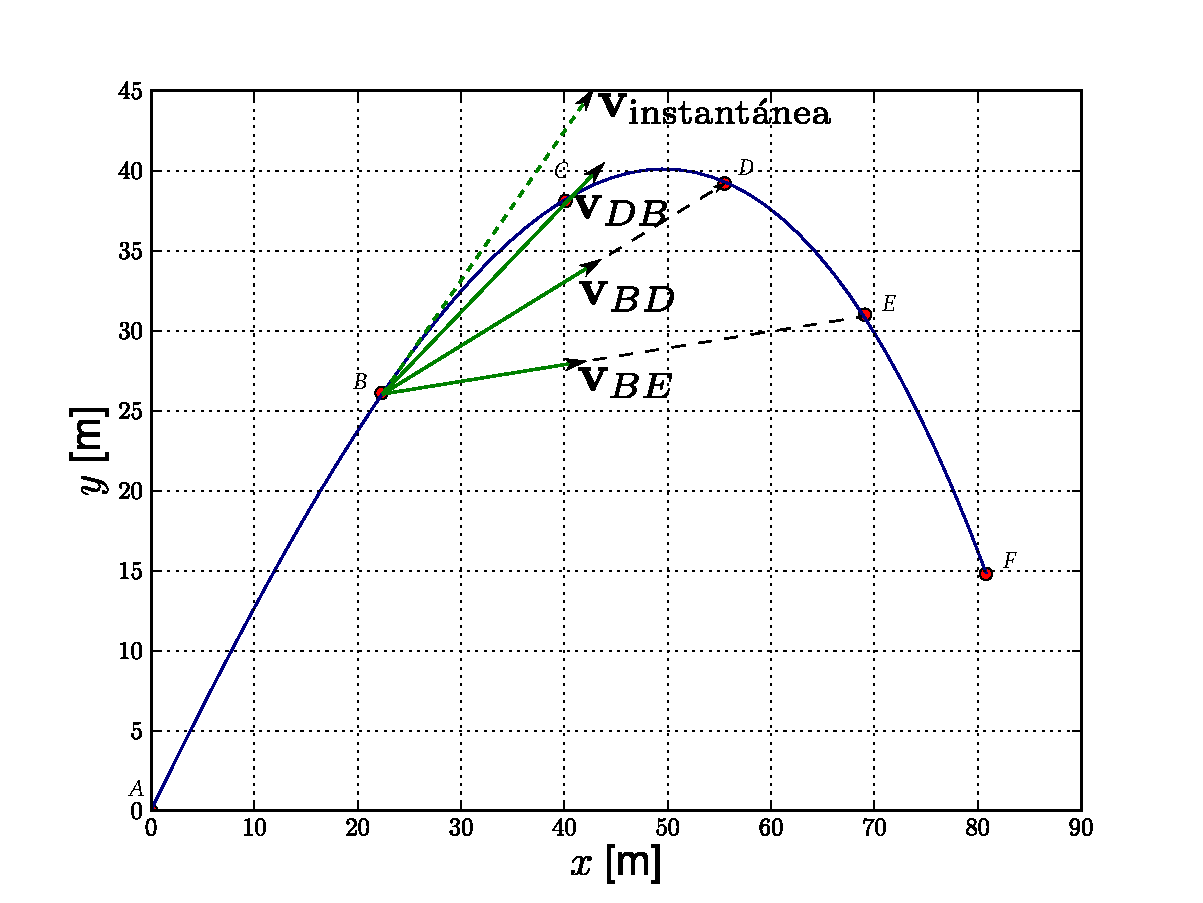
\includegraphics[scale=0.6]{flyingball8}
  \caption{Moviemto de una bola}
  \label{fig:flyingball8}
\end{figure}


La velocidad $\mathbf{v}$ de la part\'\i cula a medida que \'esta se mueve a lo largo de una trayectoria se define como
\begin{align}
  \mathbf{v}=&\lim_{\Delta t\to0}\frac{\Delta\mathbf{r}}{\Delta t}\nonumber\\
  &=\frac{d\mathbf{r}}{dt}\,,
\end{align}
que es equivalente a las ecuaciones escalares
\begin{align}
  v_x=&\lim_{\Delta t\to0}\frac{\Delta x}{\Delta t}=\frac{dx}{dt}\nonumber\\
  v_y=&\lim_{\Delta t\to0}\frac{\Delta y}{\Delta t}=\frac{dy}{dt}\nonumber\\
  v_z=&\lim_{\Delta t\to0}\frac{\Delta z}{\Delta t}=\frac{dz}{dt}\,.
\end{align}

La notaci\'on vectorial permite describir el movimiento en tres dimensiones con una sola ecuaci\'on, una econom\'\i a muy grande comparada con las tres ecuaciones que tocar\'\i a escribir si se tuviese que hacer de otro modo. 

Alternativamente, ya que $\mathbf{r}=x\hat{\mathbf{i}}+
y\hat{\mathbf{j}}+z\hat{\mathbf{k}}$, obtenemos por simple
diferenciaci\'on que (los vectores unitarios pueden cambiar bajo
diferenciaci\'on en otros sistemas de coordenadas diferentes al
cartesiano)
\begin{align}
 \frac{d\mathbf{r}}{dt}=&\frac{dx}{dt}\hat{\mathbf{i}}   
+\frac{dy}{dt}\hat{\mathbf{j}}   +\frac{dz}{dt}\hat{\mathbf{k}}\nonumber\\
=&
\left(
\frac{dx}{dt},\frac{dy}{dt},\frac{dz}{dt}
\right)\nonumber\\
=&(v_x,v_y,v_z)
\end{align}
%como antes.




En el l\'\i mite $\Delta t\to0$, $\Delta\mathbf{r}$ se convierte en la tangente a la trayectoria, como se \'\i ndica en la figura~\cite{fig:tangente}. Sin embargo, la relaci\'on
\begin{align}
  \Delta\mathbf{r}\approx&\frac{d\mathbf{r}}{dt}\Delta t\nonumber\\
  \Delta\mathbf{r}=&\mathbf{v}\Delta t,
\end{align}
que llega a ser exacta en el l\'\i mite $\Delta t\to 0$, muestra que $\mathbf{v}$ es paralelo a $\Delta\mathbf{r}$; la velocidad instant\'anea $\mathbf{v}$ de una part\'\i cula es en todas partes tangente a la trayectoria. 
\begin{figure}
  \centering
  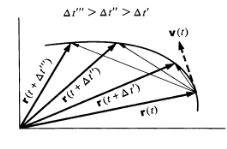
\includegraphics[scale=0.55]{tangente}
  \caption{Velocidad como tangente (Sec 1.6~\cite{Kleppner})}
  \label{fig:tangente}
\end{figure}

\begin{itemize}
\item[Ejemplo] \textbf{Encontrando $\mathbf{v}$ de $\mathbf{r}$}\\
La posici\'on de una part\'\i cula est\'a dada por
\begin{align}
  \mathbf{r}=A(e^{\alpha t}\hat{\mathbf{i}}+e^{-\alpha t}\hat{\mathbf{j}})\,,
\end{align}
donde $\alpha$ es constante. Encuentre la velocidad y bosqueje la trayectoria.
\begin{align}
    \mathbf{v}=&\frac{d\mathbf{r}}{dt}\nonumber\\
    =&A(\alpha e^{\alpha t}\hat{\mathbf{i}}-\alpha e^{-\alpha t}\hat{\mathbf{j}})\,,
\end{align}
o
\begin{align}
  v_x=&A\alpha e^{\alpha t}\nonumber\\
  v_y=&-A\alpha e^{-\alpha t}\,.
\end{align}
La magnitud de $\mathbf{v}$ es
\begin{align}
  v=&\sqrt{v_x^2+v_y^2}\nonumber\\
  =&A\alpha\sqrt{e^{2\alpha t}+e^{-2\alpha t}}\,.
\end{align}

\begin{inprogress}
  Pasar los ejemplo de MI desarrollados en el cuaderno
\end{inprogress}
En describir el movimiento de un punto, es usualmente \'util considerar los casos l\'\i mite:
\end{itemize}

\subsection{Aceleración}

Aceleración promedio:
\begin{align}
  \mathbf{a}_{\text{prom}}=&\frac{\Delta \mathbf{v}}{\Delta t}
\end{align}

Aceleración instantánea
\begin{align}
  \mathbf{a}_{\text{prom}}=&\lim_{\Delta t\to 0}\frac{\Delta \mathbf{v}}{\Delta t}=\frac{d\mathbf{v}}{dt}
\end{align}

\subsection{Moméntum}

Momentúm o cantidad de movimiento instáneo de una partícula de masa $m$ moviendo con velocidad instantánea $\mathbf{v}$
\begin{align}
  \mathbf{p}=&\gamma m \mathbf{v}\,, &\text{donde: } \gamma=&\frac{1}{\sqrt{1-\frac{|\mathbf{v}|^2}{c^2}}}\,,
\end{align}
y $c\approx 3\times 10^8\ $m/s es la velocidad de la luz.

Si $\gamma\approx1$, o equivalentemente, si $|\mathbf{v}|\ll c$, 


%%% Local Variables: 
%%% mode: latex
%%% TeX-master: "mecanica"
%%% End: 
